\documentclass{beamer}

%% \documentclass[handout]{beamer}
%% % use this with the [handout] option to create handouts for the audience
%% \usepackage{pgfpages}
%% \pgfpagesuselayout{2 on 1}[a4paper,border shrink=5mm]

\mode<presentation>
{
  \usetheme{Diku}
% set this to your preferences:
  \setbeamercovered{invisible}
%  \setbeamercovered{transparent}
}

\usepackage{graphicx}
\usepackage{epic}

\usepackage{amsmath}
\usepackage{amssymb}
\usepackage{amsthm}

\newcommand{\basetop}[1]{\vtop{\vskip-1ex\hbox{#1}}}
\newcommand{\source}[1]{\let\thefootnote\relax\footnotetext{\scriptsize\textcolor{kugray1}{Source: #1}}}

% for coloured code citation in text:
\usepackage{fancyvrb}

%%%%%%%%%%%%%%%%%%%%%%%%%%%%%%%%%
%%%%%    code sections   %%%%%%%%
%%%%%%%%%%%%%%%%%%%%%%%%%%%%%%%%%

% code highlighting commands in own block
\DefineVerbatimEnvironment{code}{Verbatim}{fontsize=\scriptsize}
\DefineVerbatimEnvironment{icode}{Verbatim}{fontsize=\scriptsize}

% Fancy code with color commands:
\DefineVerbatimEnvironment{colorcode}%
        {Verbatim}{fontsize=\scriptsize,commandchars=\\\{\}}

%%%%%%%%%%%%%%%%%%%%%%%%%%%%%%%%%%
%%%%%    some coloring    %%%%%%%%

\definecolor{Red}{RGB}{220,50,10}
\definecolor{Blue}{RGB}{0,51,102}
\definecolor{Yellow}{RGB}{102,51,0}
\definecolor{Orange}{RGB}{178,36,36}
\definecolor{Grey}{RGB}{180,180,180}
\definecolor{Green}{RGB}{20,120,20}
\definecolor{Purple}{RGB}{160,50,100}
\newcommand{\red}[1]{\textcolor{Red}{{#1}}}
\newcommand{\blue}[1]{\textcolor{Blue}{{#1}}}
\newcommand{\yellow}[1]{\textcolor{Yellow}{{#1}}}
\newcommand{\orange}[1]{\textcolor{Orange}{{#1}}}
\newcommand{\grey}[1]{\textcolor{Grey}{{#1}}}
\newcommand{\green}[1]{\textcolor{Green}{{#1}}}
\newcommand{\purple}[1]{\textcolor{Purple}{{#1}}}




% use "DIKU green" from our color theme for \emph
\renewcommand{\emph}[1]{\textcolor{structure}{#1}}
% use some not-too-bright red for an \emp command
\definecolor{DikuRed}{RGB}{130,50,32}
\newcommand{\emp}[1]{\textcolor{DikuRed}{ #1}}
\definecolor{CosGreen}{RGB}{10,100,70}
\newcommand{\emphh}[1]{\textcolor{CosGreen}{ #1}}
\definecolor{CosBlue}{RGB}{55,111,122}
\newcommand{\emphb}[1]{\textcolor{CosBlue}{ #1}}
\definecolor{CosRed}{RGB}{253,1,1}
\newcommand{\empr}[1]{\textcolor{CosRed}{ #1}}

\newcommand{\mymath}[1]{$ #1 $}
\newcommand{\myindx}[1]{_{#1}}
\newcommand{\myindu}[1]{^{#1}}

\newtheorem{mydef}{Definition}
\newtheorem{mytheo}{Theorem}
\newtheorem{mylemma}{Lemma}


%%%%%%%%%%%%%%%%%%%%

\title[Intro]{PMPH Introduction: Course Organization, Hardware Trends, List Homomorphism}

\author[C.~Oancea]{Cosmin E. Oancea\\{\tt cosmin.oancea@diku.dk}}

\institute{Department of Computer Science (DIKU)\\University of Copenhagen}


\date[Sept 2019]{September 2019 PMPH Lecture Slides}


\begin{document}

\titleslide


%%%%%%%%%%%%%%%%%%%%%%%%%%%%%%%%%%%%%%%%%%%%%%%%%%%%%%%%%%%%%%%%%%%%%%
%%%%%%%%%%%%%%%%%%%%%%%%%%%%%%%%%%%%%%%%%%%%%%%%%%%%%%%%%%%%%%%%%%%%%%
%%%%%%%%%%%%%%%%%%%%%%%%%%%%%%%%%%%%%%%%%%%%%%%%%%%%%%%%%%%%%%%%%%%%%%
%\begin{frame}[fragile]
%	\tableofcontents
%\end{frame}

%%%%%%%%%%%%%%%%%%%%%%%%%%%%%%%%%%%%%%%%%%%%%%%%%%%
%%%%%%%%%%%%%%%%%%%%%%%%%%%%%%%%%%%%%%%%%%%%%%%%%%%
%%%%%%%%%%%%%%%%%%%%%%%%%%%%%%%%%%%%%%%%%%%%%%%%%%%

\begin{frame}[fragile,t]
\frametitle{Intended Learning Outcomes}

List Homomorphism: a way of writing inherently-parallel programs.
\bigskip

\begin{itemize}
    \item explain when and where PMPH'18 lectures and lab sessions 
            are located in space and time, \bigskip

    \item explain Moore's law and argue based on hardware trends 
            and technological constraint
            why all modern and future architectures (will)
            adopt some form of massive parallelism,\bigskip

    \item explain what a list-homomorphic program is, and 
    \item be able to apply it to build programs;
    \item illustrate and apply the 1$^{st}$ Theorem of List Homomorphism 
                to transform said programs into inherently parallel ones.
\end{itemize}
\end{frame}


\begin{frame}[fragile]
	\tableofcontents
\end{frame}

\section{Brief History: Parallelism Paves the Path to Higher Performance}

\begin{frame}[fragile,t]
\frametitle{Trend towards Ever-Increasing Hardware Parallelism}

\emp{\bf Moore's Law (1960s)}
\begin{itemize}
        \item ``Number of transistors in a dense integrated circuit doubles approximatively 
                    every two years.''\pause\bigskip
        \item Rephrased as:\medskip
            \begin{itemize}
                \item computing power doubles every 19-24 months, and 
                \item cost effectiveness ({\tt performance/cost}) keeps pace.
            \end{itemize}\bigskip
\end{itemize}

\emp{\bf Brief History}
\begin{itemize}
        \item \emph{ICPP, ISCA (1980/90s): parallel architectures popular topic.}\bigskip
                %\\Demise of SingleCPU System: inevitable \& fast approaching.\bigskip

        \item \alert{Whatever happened? Mid90 Killer-Micro:}\pause
        \begin{itemize}
            \item path of least resistance: ever increasing the speed of Single CPU
            %\item Muscled processors executing 100s instructions/cycle.
            \item Commercial arena: multiprocessors just an uniprocessor extension.
        \end  {itemize}\bigskip

        \item \emph{What Changed?} Multiprocessors Trend: Academia \& Industry:
        \begin{itemize}
            \item \emph{power complexity} $P_{dynamic} \sim Freq^3$. \alert{Example!}\pause
            \item \emph{Memory WALL}: ever-increasing performance gap between 
                                        processor \& memory 
        \end  {itemize}\bigskip

%       \item \emph{All Future Architectures adopt some form of massive parallelism!}
\end{itemize}

\end{frame}

\begin{frame}[fragile,t]
\frametitle{Processor: Clock Frequency/Rate}

1990-2004: clock rate has increased exponentially.

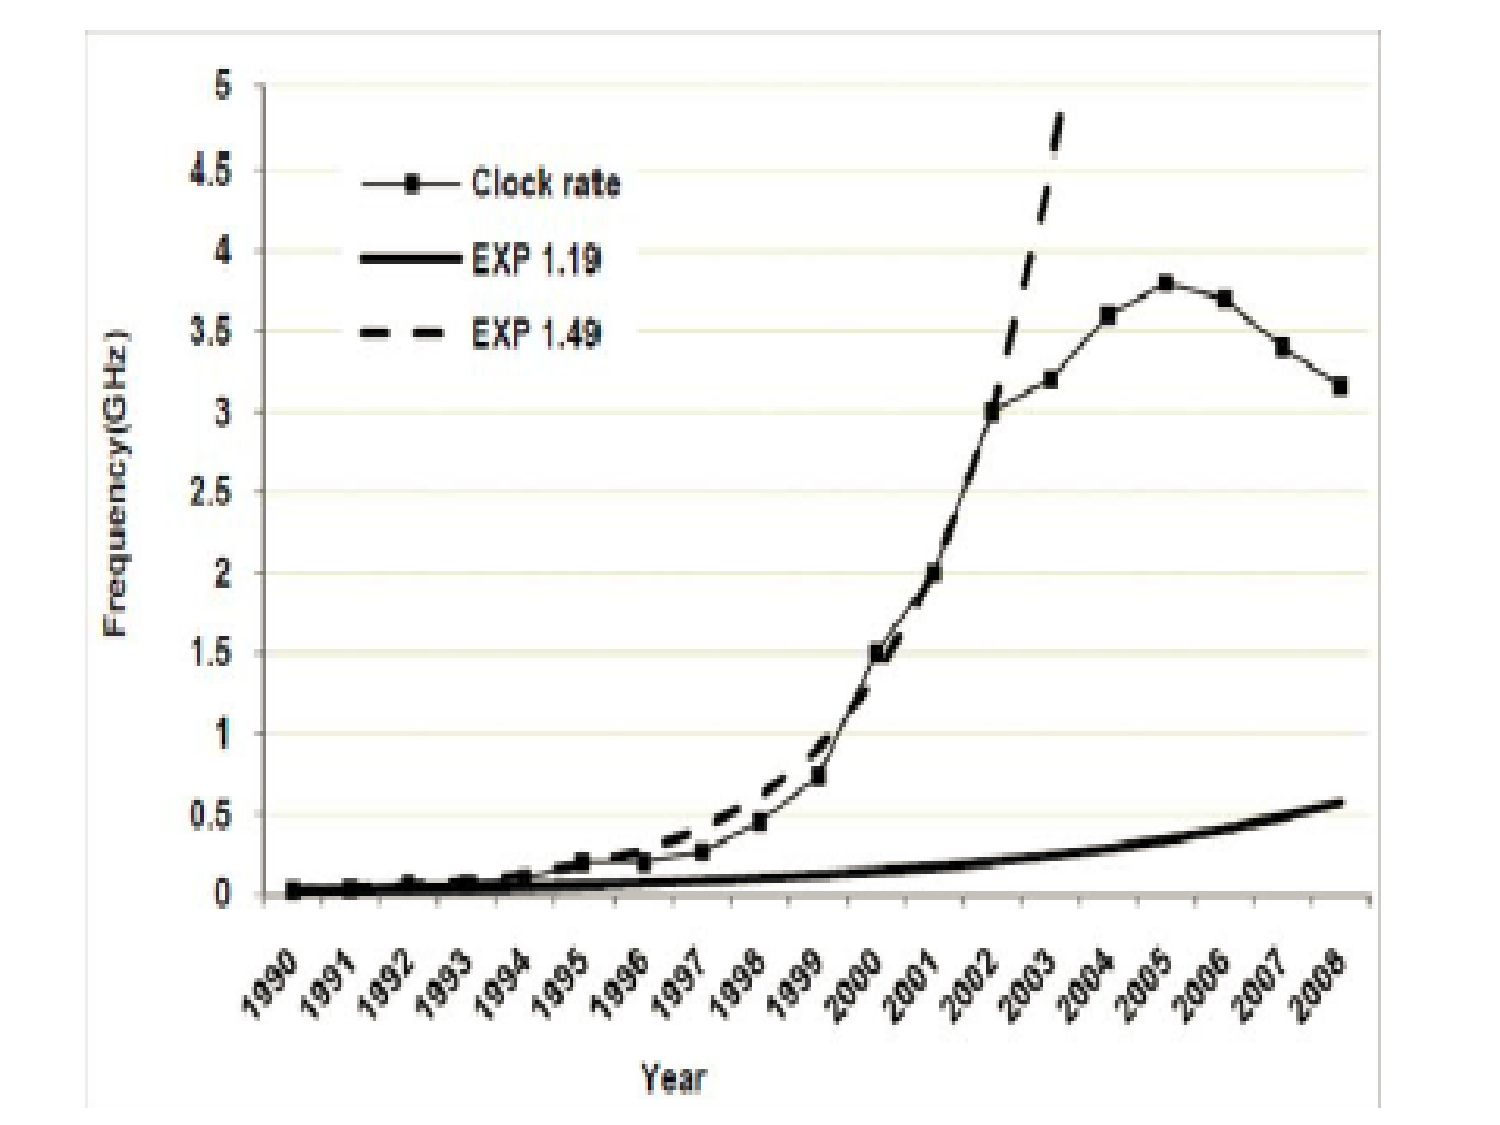
\includegraphics[width=47ex]{Figures/L1/FreqGraph}

2004: Intel cancels Pentium4 @4Ghz and shifts focus to multi-cores.

\end{frame}


\begin{frame}[fragile,t]
\frametitle{Memory Wall? Which Memory Wall??}

\begin{columns}
\column{0.65\textwidth}
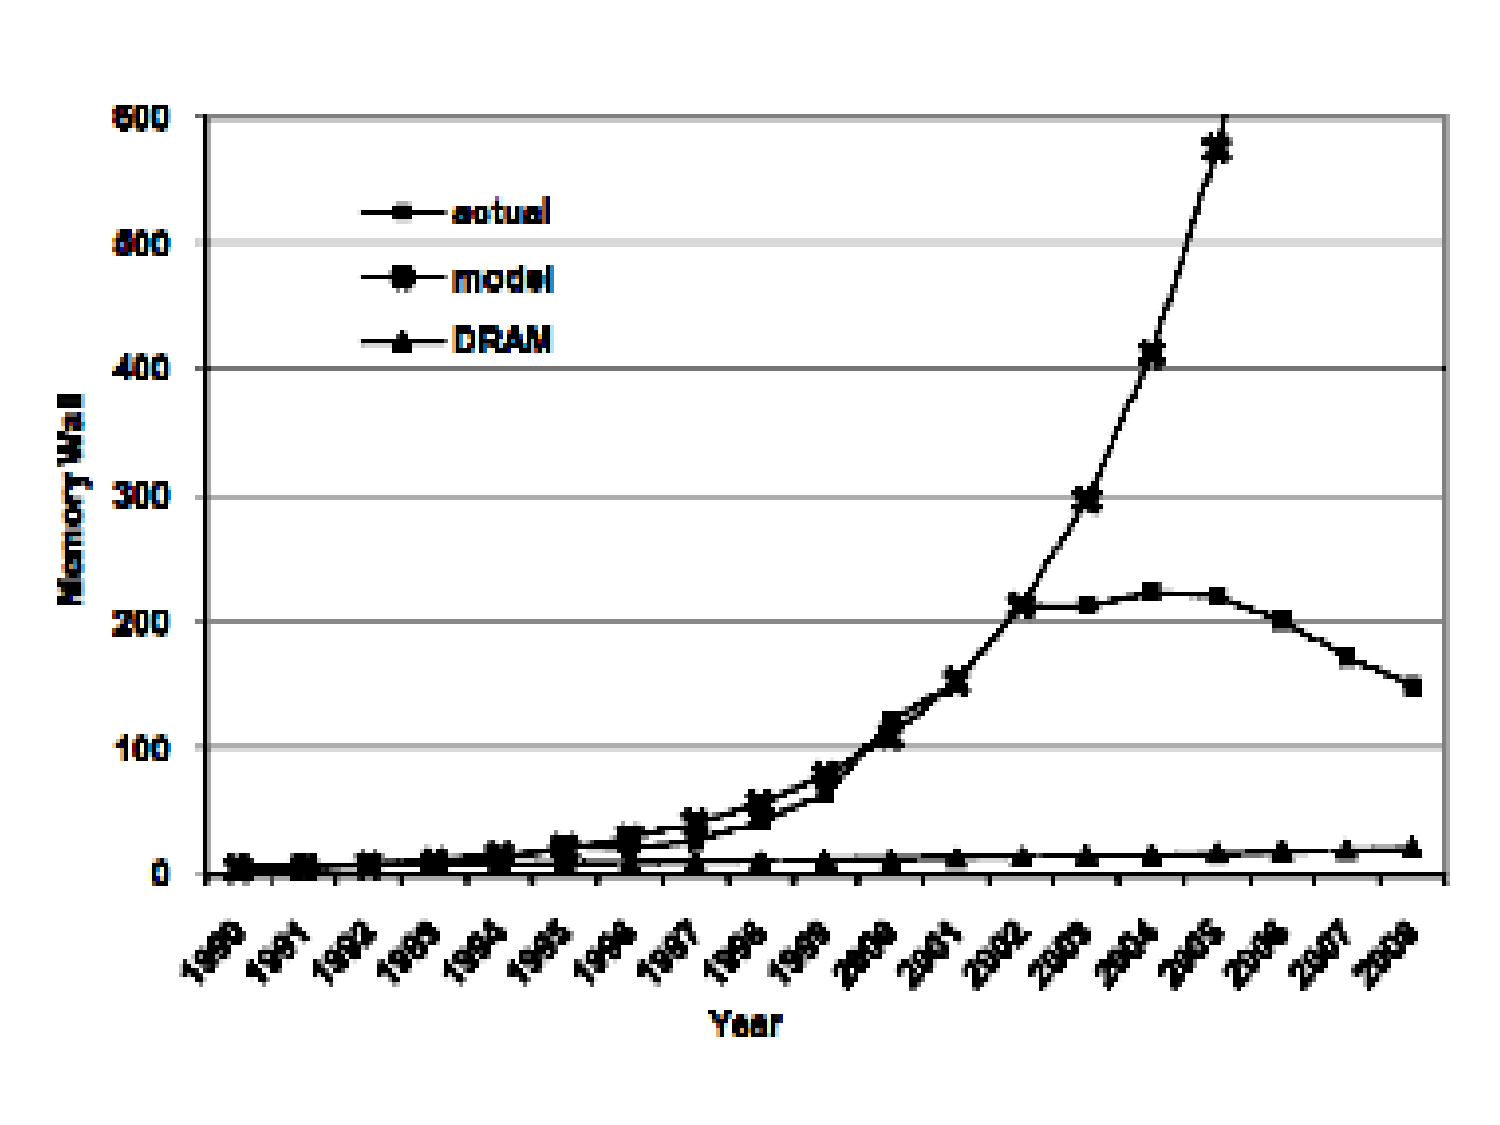
\includegraphics[width=50ex]{Figures/L1/MemWall}
\column{0.3\textwidth}
\begin{scriptsize}
\begin{itemize}
\item {\tt MemoryWall = mem\_cycle/ proc\_cycle} \smallskip
\item[1990] {\tt MemoryWall = 4} (25MHz,150ns)
\item[2002] exponential growth {\tt MemoryWall = 200} 
\item Stalled since then.
\end{itemize}
\end{scriptsize}
\end{columns}

\end{frame}


\begin{frame}[fragile,t]
\frametitle{Biggest Challenge For Parallel Hardware}

\bigskip

\includegraphics[width=29ex]{Figures/L1/Synergy}
\bigskip\pause


\emp{Important Juncture:}\medskip
\begin{itemize}
            \item \emph{Trend Today: the number of cores grows exponentially.}\medskip
            \item \alert{Biggest Challenge: develop efficient Massively-Parallel Software!}\medskip
            \item think programs with parallelism in mind rather 
                    than hack \alert{some} parallelism out of a sequential implementation.
\end  {itemize}
\end{frame}


\section{Course Organization}

\begin{frame}[fragile]
	\tableofcontents[currentsection]
\end{frame}

\begin{frame}[fragile]
\frametitle{When and Where?}
    Lectures+Lab Time and Place:\bigskip
    \begin{itemize}
        \item Tuesday 10:00am - 12:00, Aud 03, Universitetsparken 5, HCØ\medskip
        \item Thursday 10:00 - 12:00, 13:00 - 17:00 pm:\medskip
            \begin{itemize}
                \item Lecture: 10:00 - 12:00  ov-3-1-25, Universitetsparken 1-3, DIKU
                \item Lab (weeks 36-39): 13:00 - 17:00, Aud 03 (AKB), Universitetsparken 13
                \item Lab (weeks 40-44): 13:00 - 17:00, Aud D, Blegdamsvej 15-21
            \end{itemize}
        \item \red{Office hours?}
    \end{itemize}  
\end{frame}

\begin{frame}[fragile]
\frametitle{Tentative Lecture/Lab Schedule}

Your TA: Einar Rasmussen, ftc208@alumni.ku.dk,\\
(mainly grading assignments and moderate Absalon discussions)\bigskip

Cosmin will lead the lectures + lab.\bigskip

Continuous-evaluation assessment:
\begin{itemize}
    \item four individual weekly assignments: $40\%$ of final grade\medskip
    \item one group project + final presentation and discussion: $60\%$ of final grade.
        \begin{itemize}
            \item you may chose from multiple possible projects
            \item presented tentatively during Lab on Thursdays
            \item or discuss your own project with me.
            \item projects can be very practical in CUDA, Futhark, or more theoretical.
        \end{itemize}
\end{itemize} 
\end{frame}

\begin{frame}[fragile]
\frametitle{What does PMPH studies?}

Hardware track studies the design space of the critical components of parallel hardware:\medskip
    \begin{itemize}
        \item processor (ILP, intra and inter-core)\smallskip
        \item memory hierarchy (coherency)\smallskip
        \item interconnect (inter-cores or core-cache routing)\smallskip
    \end{itemize}
\bigskip
\pause

Software track studies programming models for expressing data parallelism + way to reason and optimize parallelism:\medskip
    \begin{itemize}
%        \item we focus on data parallelism since it scales 
        \item High-level of abstraction:\\ 
                list-homomorphism $\equiv$ functional map-reduce style + flattening\smallskip
        \item Low-level of abstraction:\\
                loops and transformations rooted in data dependency analysis\smallskip
        \item Lecture Notes are available for the software track!
    \end{itemize}
\bigskip
\pause

Lab track applies in practice various optimizations/transformations learned on the software track.

\end{frame}


%%%%%%%%%%%%%%%%%%%%%%%%%%%%%%%%%%%%%%%%%%%%%

\section{Hardware Trends of Critical Components of a Parallel System}

\begin{frame}[fragile]
	\tableofcontents[currentsection]
\end{frame}

\subsection{Processor}

\begin{frame}[fragile,t]
\frametitle{Abstractions}
\medskip

\begin{itemize}
%    \item[Program] set of statements performing computational steps.
%    \item[Process/Thread] embeds the execution of the computation.
    \item A \emp{program} is to a \emp{process/thread} 
            what a recipe is for cooking.\smallskip

    \item \emp{Processor (core)}: hardware entity capable of
            sequencing \& executing thread's instructions.\smallskip

    \item \emp{MT Cores} multiple threads, each 
            running in its thread context.\smallskip

    \item \emp{Multiprocessor:} set of processors connected to execute a workload
        \begin{itemize}
            \item mass produced, off-the-shelf, each several cores \& levels of cache
            \item trend towards migrating system functions on the chip:\\
                    memory controllers, external cache directories, network interface
        \end  {itemize}
\end{itemize}

%\begin{columns}
%\column{0.33\textwidth}
%\includegraphics[width=29ex]{Ch1Figs/Synergy}
%\column{0.63\textwidth}\vspace{-3ex}
%\begin{itemize}
%    \item Computer Architect Role:
%    \item \emp{design trade-offs across HW/SW interf to meet functional 
%            \& performance requirements within cost constraints.}
%\end{itemize}
%\end{columns}

\end{frame}


\begin{frame}[fragile,t]
\frametitle{Processor: Clock Frequency/Rate}

Historically the clock rate (at which instr are executed) has increased 
exponentially (1990-2004).

\begin{columns}
\column{0.65\textwidth}
\hspace{-5ex}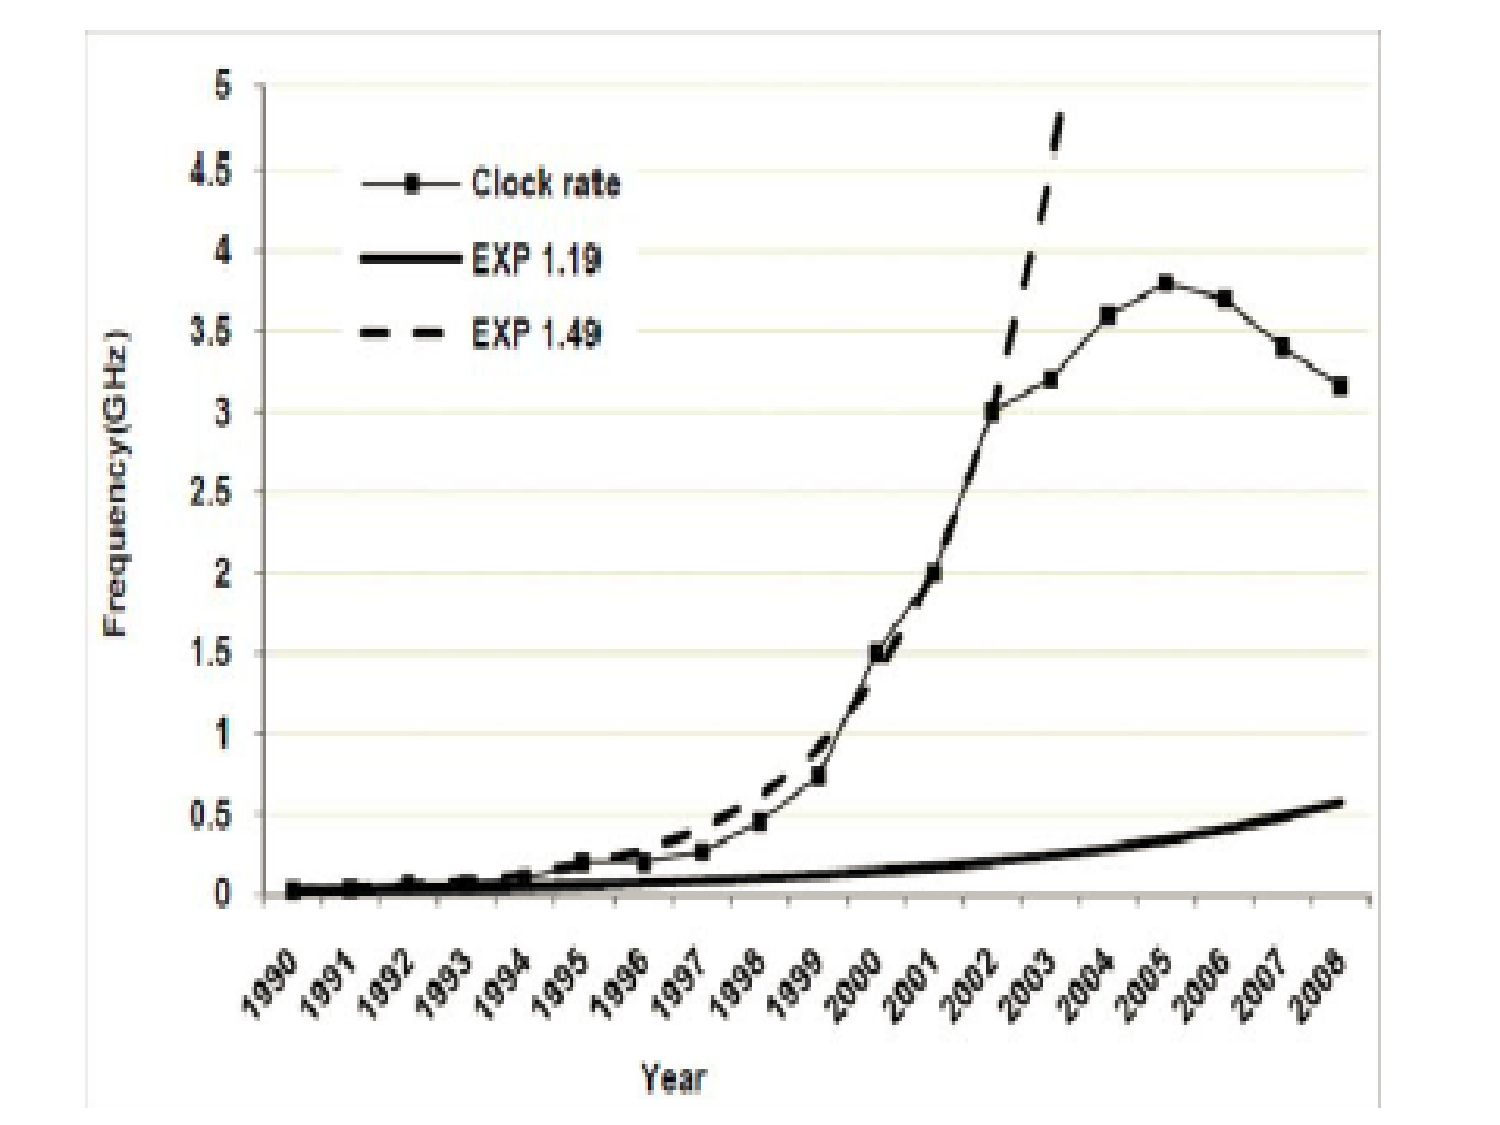
\includegraphics[width=52ex]{Figures/L1/FreqGraph}\pause
\column{0.48\textwidth}\vspace{-3ex}
\begin{scriptsize}
        \begin{itemize}
            \item $1.19\times$ per-year due technology scaling
                    (same hwd on new techn).

            \item 1990-2002: doubled every $21$ months
                    \alert{Curve $1.49\times$: $30$GHz in 2008!}
            
            \item $1.49\times - 1.19\times$: very-deep (10-20 stages) pipelines!
                    ILP via speculative OoO: register renaming, 
                        reorder buffs, branch prediction, 
                        lockup-free caches, memory disambiguation, etc. 

            \item 2004: Intel cancels Pentium4 @4Ghz \&
                    \emph{Switched Track to Multi-Cores} $\Rightarrow$\\
                    \alert{Tectonic Shift away from muscled deeply-pipelined 
                    uniprocessor.}

            \item \emp{Peaked in 2005, but mostly stalled since 2002!}
                     
        \end  {itemize}
\end{scriptsize}
\end{columns}

\end{frame}


\begin{frame}[fragile,t]
\frametitle{Closer Look at Clock Rate}

\begin{columns}
\column{0.5\textwidth}
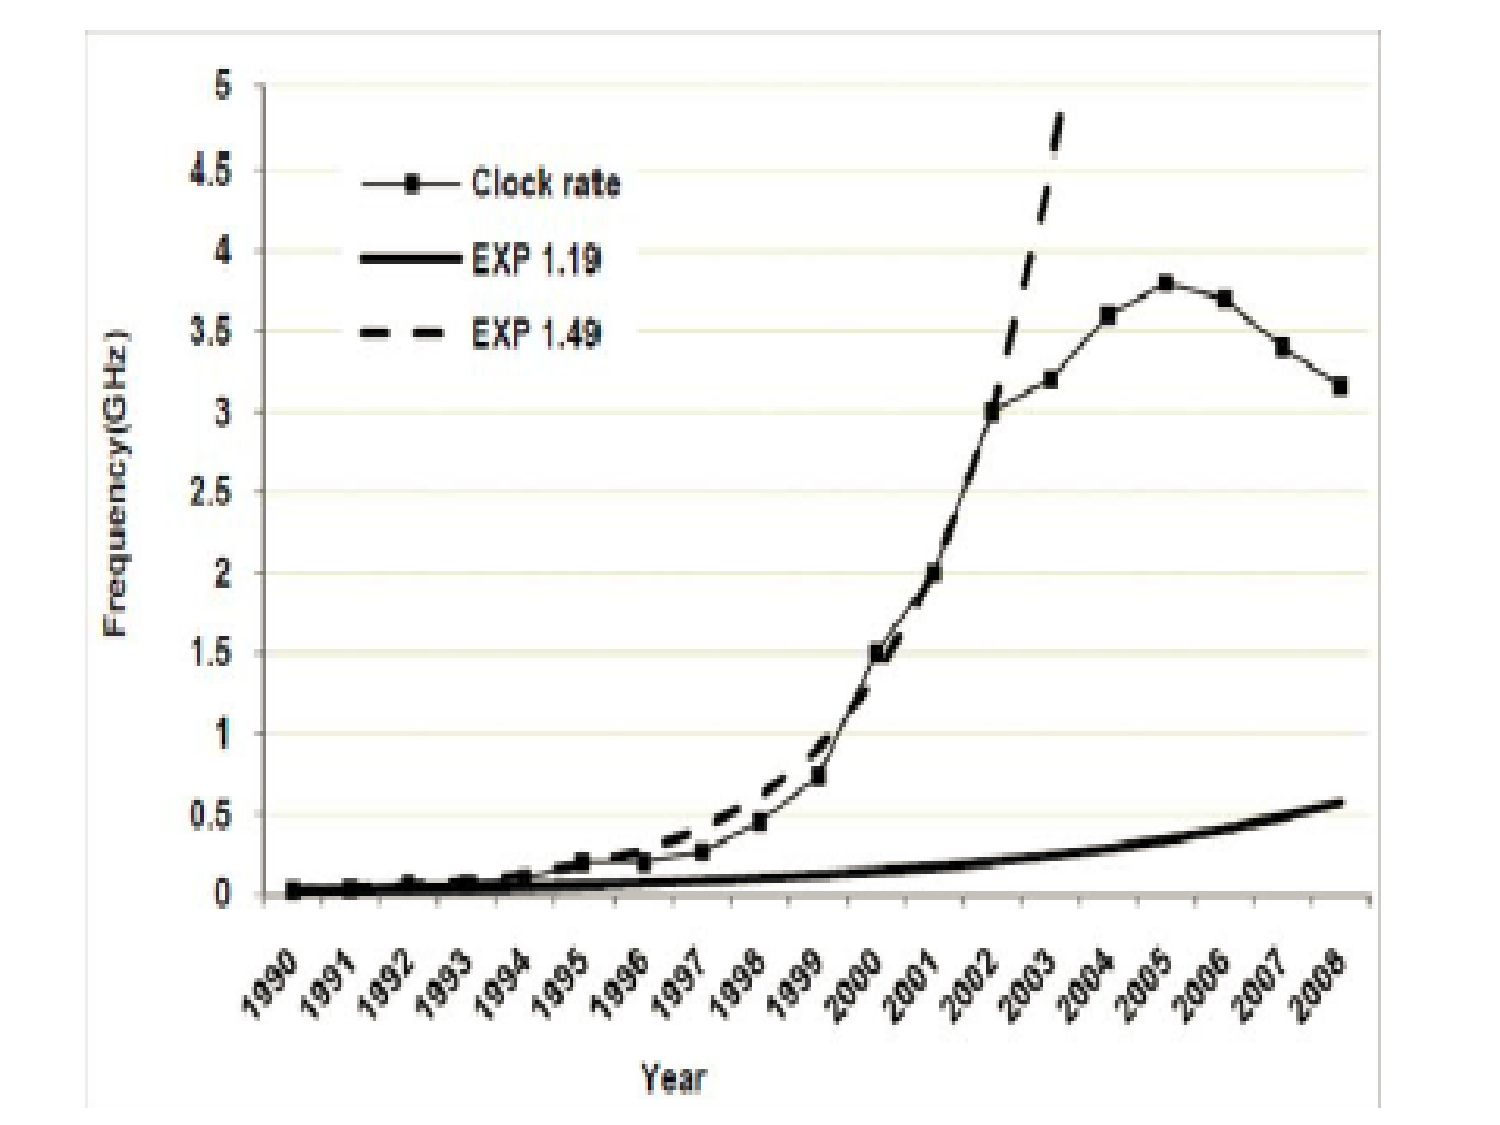
\includegraphics[width=40ex]{Figures/L1/FreqGraph}
\column{0.57\textwidth}
        \begin{itemize}
            \item \emph{Technology} (process shrinkage): every generation 
                    transistors' \emph{switching speed increases $41\%$}.\medskip

%                    \item Impact blunted in the future due to \emp{wire delays}
%                                (do not scale)
%                            because speed of wire transmission grows much slower than
%                            switching speed.
%                \end  {itemize}\medskip
            \item \emph{Pipeline Depth:} more stages $\Rightarrow$
                            less complex $\Rightarrow$ less gates/stage
                \begin{itemize}
                    \item \# of gates delays dropped by $25\%$ every process generation.
                \end  {itemize}\medskip

                \item \emph{Improved Circuit Design} 
        \end  {itemize}\bigskip
\end{columns}
\pause

Clock Rate Increase is Not Sustainable:
\begin{itemize}
    \item \emp{Deeper pipelines}: difficult to build useful stages with $<$ 10 gates
    \item \emp{Wire delays:} wire-transm speed $\uparrow$ much 
            slower than switching,
    \item Circuits clocked at \emp{higher rates consume more power}!  
\end  {itemize}

\end{frame}

\begin{frame}[fragile,t]
\frametitle{Processor: Feature Size \& Number of Transistors}

\begin{columns}
\column{0.65\textwidth}
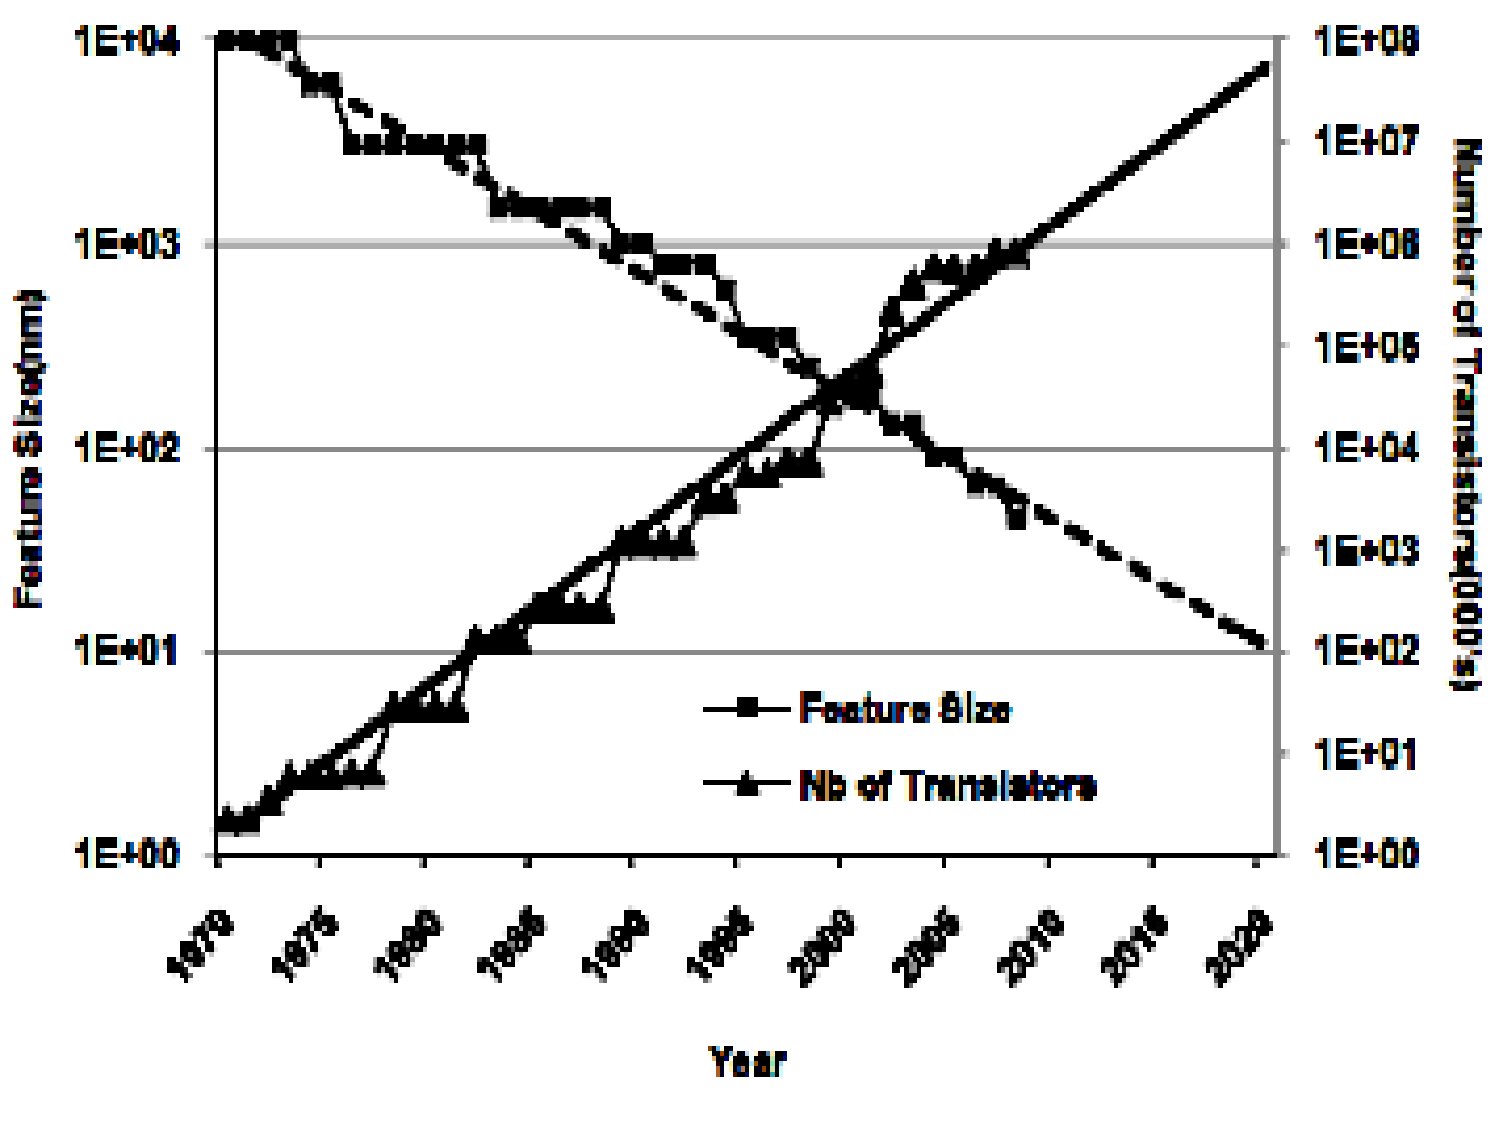
\includegraphics[width=47ex]{Figures/L1/FeatureSize}
\column{0.4\textwidth}
%\begin{scriptsize}
        \begin{itemize}
            \item new process generation every 2 years\smallskip
                
            \item feature size reduced $30\%$ every generation

            \item \# of transistors doubles every 2 years (Moore's low).\\
                    1 Billion in 2008. 
        \end  {itemize}
%\end{scriptsize}
\end{columns}
\vspace{-2ex}

Each process generation offers new resources.
\emp{How best to use the $>100$ billion transistors? Large-Scale CMPs (100s-1000s cores)}:
\begin{itemize}
    \item more cache, better memory-system design
    \item fetch and decode multiple instr per clock
    \item running multiple threads per core and on multiple cores
\end  {itemize} 

\end{frame}

\subsection{Memory}

\begin{frame}[fragile,t]
\frametitle{Memory Systems}

\begin{itemize}
    \item \emp{(Main) Memory Wall:} growing gap between processor and memory speed.
            Processor cannot execute faster than memory system can deliver data 
            and instructions!\bigskip

    \item Want Big, Fast \& Cheap Memory System\smallskip
    \begin{itemize}
        \item access time 
                increases with memory size as it is dominated by 
                wire delays$\Rightarrow$ this will not change in future technologies\smallskip
%(address decoding, address line propagation, bit-line propagation) 
        \item multi-level hierarchies (relies on principle of locality)\smallskip
        \item efficient management is KEY, e.g., cache coherence.\smallskip
        \item Cost and Size memories in a basic PC in 2008:
    \end  {itemize} 
\end{itemize}
\bigskip

\begin{tabular}{|l|l|l|l|l|}\hline
Memory & Size  & Marginal Cost & Cost Per MB & Access Time \\\hline
L2 Cache & 1MB & \$20/MB & \$20 & 5nsec \\\hline
Main Memory & 1 GB & \$50/GB & 5c & 200 nsec \\\hline
Disk & 500GB & \$100/500GB & 0.02c & 5 msec \\\hline
\end{tabular}

\end{frame}


\begin{frame}[fragile,t]
\frametitle{Memory Wall? Which Memory Wall??}

\begin{itemize}
            \item \emph{DRAM density increases $4\times$ every 3 years, BUT} \smallskip

            \item \emp{DRAM speed $\uparrow$ only with $7\%$ per year!} 
                    (processor speed by $50\%$) 

            \item \alert{Perception was that Memory Wall will last forever!}

            \item \emph{Memory Wall Stopped Growing around 2002}.
    
            \item Multi/Many-Cores $\Rightarrow$ shifted from Latency 
                    to \emp{Bandwidth WALL}
\end  {itemize}
\vspace{-3ex}

\begin{columns}
\column{0.65\textwidth}
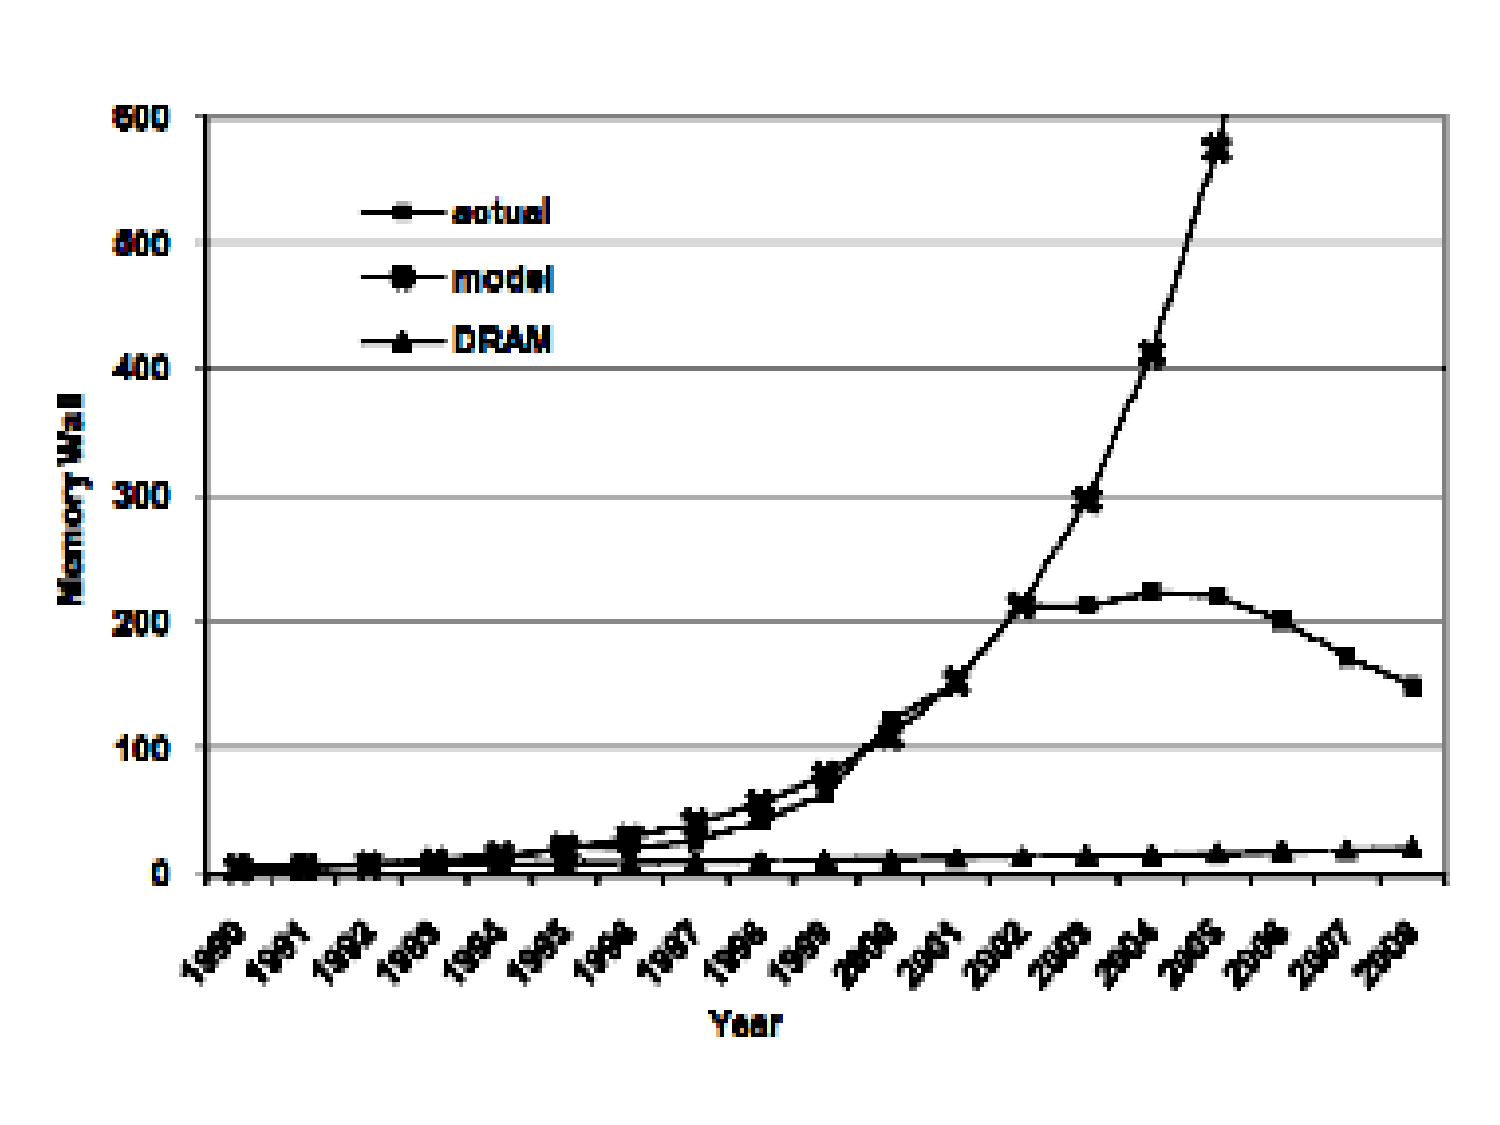
\includegraphics[width=50ex]{Figures/L1/MemWall}
\column{0.3\textwidth}
\begin{scriptsize}
\begin{itemize}
\item {\tt MemoryWall = mem\_cycle/ proc\_cycle} \smallskip
\item[1990] {\tt MemoryWall = 4} (25MHz,150ns)
\item[2002] exponential growth {\tt MemoryWall = 200} 
\item Stalled since then.
\item If trend continues: 1 Terabit Main Memory by 2021.
\end{itemize}
\end{scriptsize}
\end{columns}

\end{frame}


\begin{frame}[fragile,t]
\frametitle{Disk Memory}

\begin{itemize}
            \item \emph{Historically disk performance improved by $40\%$ per year} \smallskip

            \item {\tt DiskTime=AccessTime+TransferTime} ({\scriptsize {\tt AccessTime=Seek+Latency}})

            \item Historically, transfer time have dominated, but

            \item Today: transfer and access time are of the same \alert{msecs} order
    
            \item Future, Access Time will dominate, but proc-disk gap still large
\end  {itemize}

\begin{columns}
\column{0.5\textwidth}
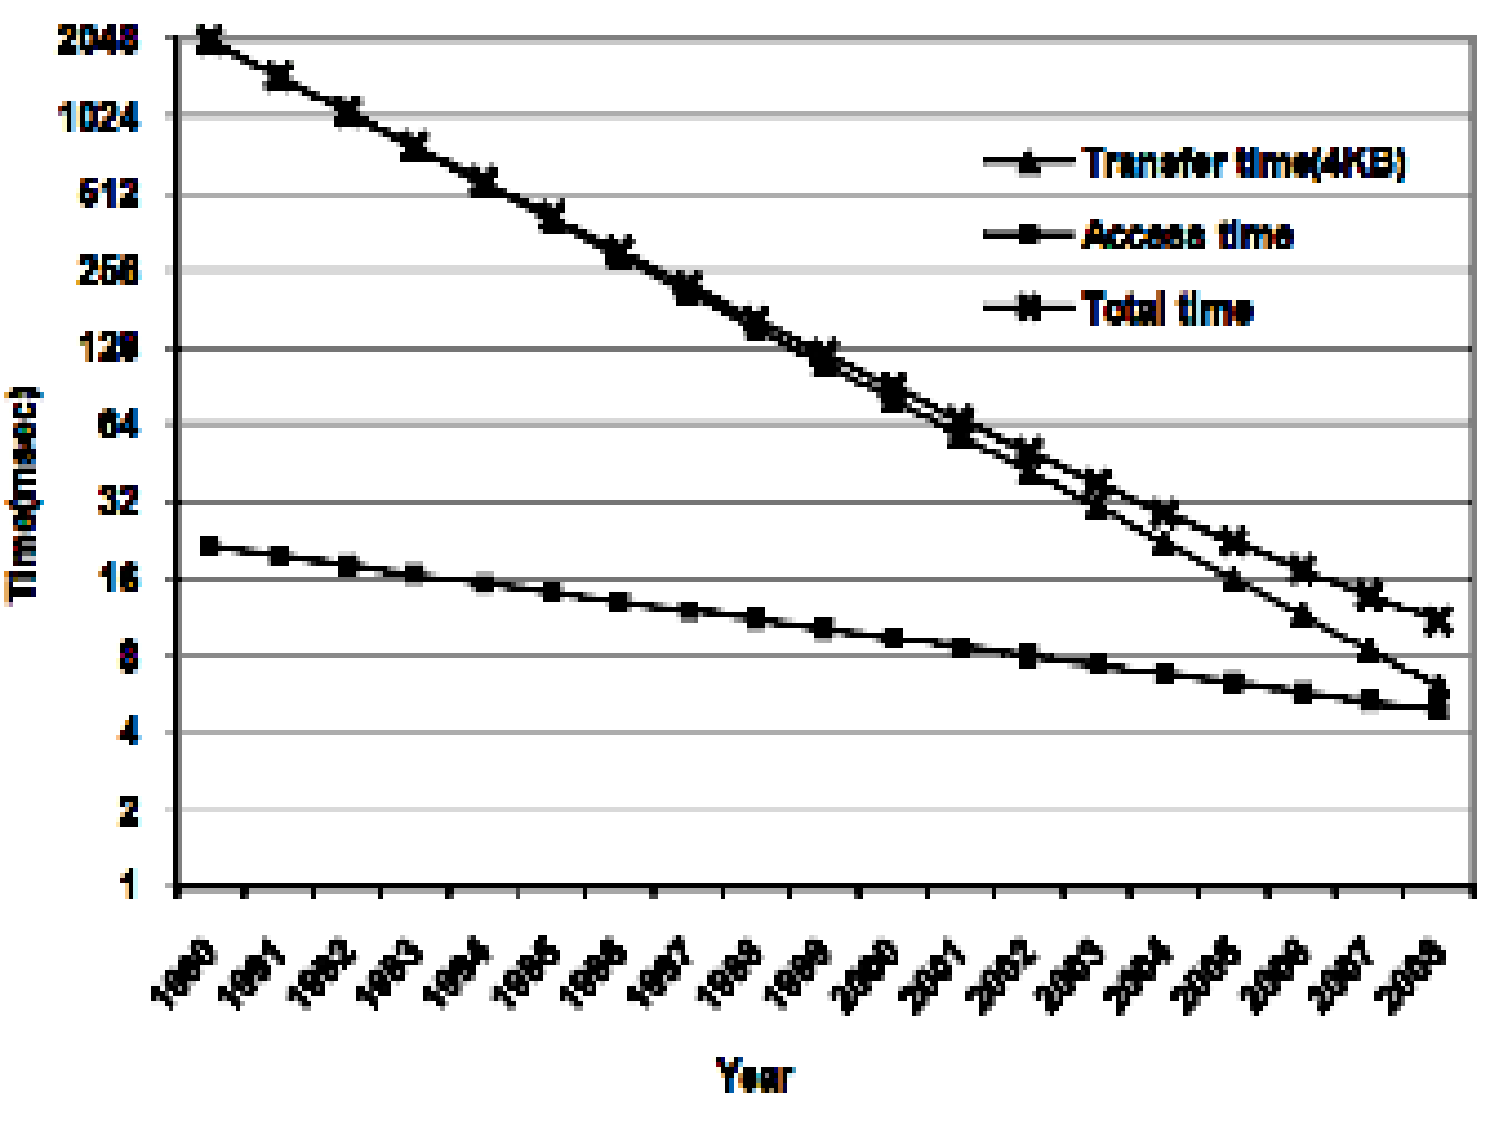
\includegraphics[width=33ex]{Figures/L1/DISK}
\column{0.5\textwidth}
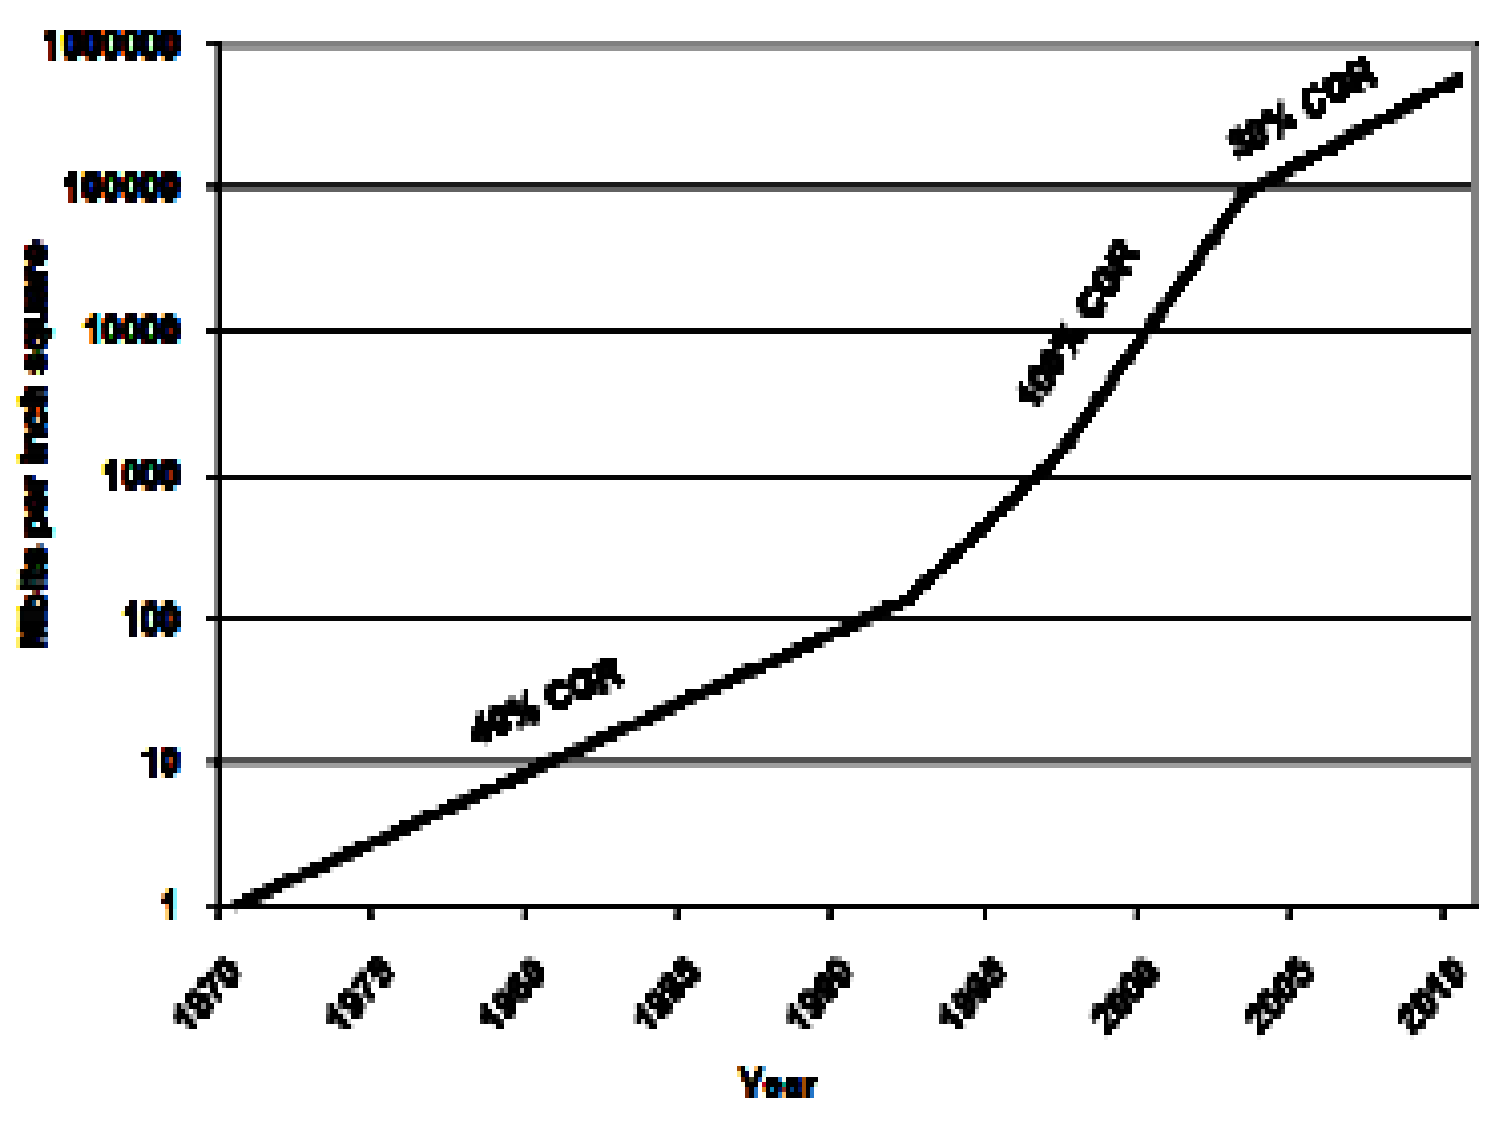
\includegraphics[width=33ex]{Figures/L1/Disk2}
\end{columns}

{\scriptsize Seek Time: head to reach right track, latency: time to reach the first record on track, both depend on rotation speed \& independent on block size}.

\end{frame}

\subsection{Interconnect}
\begin{frame}[fragile,t]
\frametitle{Interconnection Networks}

Present at many layers:
\begin{itemize}
            \item \emp{On-Chip Interconnects:} forward values between pipeline stages, AND between execution units AND connect cores to shared cache banks. \smallskip

            \item \emp{System Interconnects:} connect processors (CMPs) to memory and IO

            \item \emp{I/O Interconnects}, usually bus e.g., PCI, connect various 
                    devices to the System Bus
            \item \emp{Inter-Systems Interconnects:} connect separate systems (chassis or boxes) \& include
                \begin{itemize}
                    \item \emph{SANs:} connect systems at very short distance
                    \item LANs, WANs (not interesting for us).
                \end  {itemize}

            \item Internet: global world-wide interconnect (not interesting for us).
\end  {itemize}

\end{frame}

%%%%%%%%%%%%%%%%%%%%%%%%%%%%%%%%%%%%%%%%%%%%
%%%%%%%%%%%%%%%%%%%%%%%%%%%%%%%%%%%%%%%%%%%%

\section{Technological Challenges/Constraints}

\begin{frame}[fragile]
	\tableofcontents[currentsection]
\end{frame}


\begin{frame}[fragile,t]
\frametitle{Technological Contraints}

\begin{itemize}
    \item In the Past: tradeoff between cost (area) and time (performance).\bigskip

    \item Today: design is challenged by several technological limits\smallskip
        \begin{itemize} 
            \item \alert{Major new contraint is Power}\smallskip
            \item wire delays\smallskip
            \item reliability\smallskip
            \item complexity of design
        \end  {itemize}\bigskip

    \item \emphh{It seems that parallelism addresses well all these constraints.} 
%    \item Architecture can play a significant role to maintain viability
%            of CMOS technology for years to come.\bigskip

\end{itemize}
\end{frame}

\subsection{Power}

\begin{frame}[fragile,t]
\frametitle{Power}

\begin{itemize}
    \item \emp{\tt Total Power = Dynamic + Static (Leakage)}\\
                        $P_{dynamic} = \alpha C V^2 f$ 
                        consumed by a gate when it switches state\\
                        $P_{static}  = V I_{sub} \sim V e^{-k V_T / T}$ 
                        (caches)\\
    {\tiny $V$ supply voltage, $f$ clock rate, $\alpha$ activity factor, $\alpha f$ the rate at which gates switch, $T$ temperature}\medskip
            

    \item Dynamic power 
            favors parallel processing over higher clock rate
            \begin{itemize}
                \item $P_{dynamic} \sim f^3$ mostly dissipated in processor\pause
                \item increase clock freq $4\times$ $\Rightarrow$ \pause
                        $4\times$ speedup @ $64\times$ dynamic power!
                \item replicate a uniprocessor $4\times$ $\Rightarrow$ 
                        $4\times$ speedup @ $4\times$ power
            \end  {itemize}\medskip

    \item Static Power: dissipated in all circuits,  
                at all time, no matter of frequency and whether
                it switches or not.\\ 
            {\tiny Proportional to the area of circuit but independent of clock rates and circuit activity.}
            \begin{itemize}
                \item negligible 15 years ago, but as feature size 
                        decreased so did the threshold voltage $V_T$ 
                        every generation
                \item \alert{Recently overtook dynamic power as major 
                        source of dissipation!}
            \end{itemize}\medskip

    \item \emp{Power/Energy are Critical Problems}\\ 
                e.g., costly \& many battery operated devices.
%            \begin{itemize}
%                \item Power must be dissipated otherwise temperature
%                        goes up \& affects performance, correctness and
%                        may possibly destroy the circuit, short or long term. 
%                \item Energy depends on power and speed. Costly \& 
%                        many devices are battery-operated devices.
%
%            \end  {itemize}
\end  {itemize}


\end{frame}


\subsection{Reliability}

\begin{frame}[fragile,t]
\frametitle{Reliability}

\begin{itemize}
    \item \emp{Transient Failures (Soft Errors):}
        \begin{itemize}
            \item Corruption Sources: cosmic rays, alpha particles
                    radiating from the packaging material, electrical noise;
            \item Charge stored in a transistor \emp{\tt Q = C V}
            \item Supply voltage $V$ decreases every generation\\
                    (consequence of features-size shrinking)
            \item As Q decreases, it is easier to flip bits
            \item Device operational but values have been corrupted
            \item DRAM/SRAM error detection and correction capability
        \end  {itemize}\medskip

    \item \emp{Intermittent/Temporary Failures:}
            \begin{itemize}
                \item last longer, should try to continue execution
                \item aging or temporary environmental variation, e.g., temperature
            \end  {itemize}\medskip

    \item \emp{Permanent Failures:} device will never function again,
                must be isolated \& replaced by spare\medskip

    \item \emph{Chip Mutiprocessors: promote better reliability}
            \begin{itemize}
                \item using threads for redundant execution, 
                \item faulty cores can be disabled $\Rightarrow$ 
                        natural failsafe degradation
            \end  {itemize}
\end  {itemize}
\end{frame}

\subsection{Wire Delays}
\begin{frame}[fragile,t]
\frametitle{Wire Delays}

\begin{itemize}
    \item Miniaturization $\Rightarrow$ transistors switch faster,
            but the propagation delay of signals on wire does not 
            scale as well.\medskip

    \item Wire Delay Propagation $\sim R C$. $R \sim L / CS_{area}$.
            Miniaturization $\Rightarrow$ cross-section area keeps shrinking
                each generation, annuls the benefit of length shrinking. \medskip

    \item Wires can be pipelined like logic.\medskip

    \item Deeper pipelines are better because communication
            limited to only few stages.\medskip

    \item \emph{Impact of wire delays also favors multiprocessors,
            since communication traffic is hierarchical:}
            \begin{itemize}
                \item most communication is local 
                \item inter-core communication is occasional
            \end  {itemize}

\end  {itemize}
\end{frame}

\subsection{Design Complexity}
\begin{frame}[fragile,t]
\frametitle{Design Complexity}

\begin{itemize}
    \item Design Verification has become the dominant cost of chip
            development today, major design constraint.\medskip

    \item \emp{Chip density increases much faster than the productivity 
                of verification engineers} (new tools and speed of systems):
            \begin{itemize}
            \item register-transfer language level, i.e., logic is correct 
            \item core level, i.e., correctness of forwarding, memory disambiguation,
            \item multi-core level, e.g., cache coherence, memory consistency.
            \end  {itemize}\medskip

    \item Vast majority of chip resources dedicated to storage
            also due to verification complexity:
            \begin{itemize}
            \item trivial to increase the size of: 
                caches, store buffers, load/store/ fetch queues, reorder buffers,
                    directory for cache coherence, etc.
            \end  {itemize}\medskip

    \item \emph{Design Trend Favors Multiprocessors:}
            easier to replicate the same structure multiple times
            than to design a large, complex one.
\end  {itemize}
\end{frame}

\subsection{CMOS Endpoint}
\begin{frame}[fragile,t]
\frametitle{CMOS (Endpoint) Meets Quantum Physics}

\begin{itemize}
    \item CMOS is rapidly reaching the limits of miniaturization,\medskip

    \item Feature size: half pitch distance (half the distance between
            two metal wires). Gate length $\sim 1/2$ feature size.\medskip

    \item If present trends continues feature size $< 10 nm$ by 2020\medskip

    \item Radius of atom: $0.1 \sim 0.2 nm$ $\Rightarrow$ gate length quickly
            reaches atomic distances that are governed by quantum physics,
            i.e., binary logics replaced with probabilistic states.\medskip

    \item Not clear what will follow (?)
\end  {itemize}
\end{frame}


\section{List Homomorphisms (LH)}

\subsection{List Homomorphism Definition and 1st Theorem}

\begin{frame}[fragile]
	\tableofcontents[currentsection]
\end{frame}

\begin{frame}[fragile,t]
\frametitle{Shape of a List-Homomorphic Program (LH)}

Realm of finite lists:
\begin{itemize}
    \item {\tt ++} denotes list concatenation:\\
    {\tt [1, 2, 3] ++ [4, 5, 6, 7] $\equiv$ [1, 2, 3, 4, 5, 6, 7]}
    \item empty list {\tt []} is the neutral element:
        {\tt [] ++ x $\equiv$ x ++ [] $\equiv$ x}
\end{itemize}
\bigskip

\emp{\bf LH: a special form of divide and conquer programming:}
\begin{columns}
\column{0.44\textwidth}
\begin{colorcode}[fontsize=\small]
h [ ] = e
h [x] = f x
h (x ++ y) = (h x) \mymath{\odot} (h y)
\end{colorcode}
\pause
\alert{A well-defined program requires that no matter how 
the input list is partitioned into {\tt x ++ y}, the result is the same!}
\column{0.45\textwidth}
\begin{colorcode}[fontsize=\small]
\blue{--computes the length of a list,}
\blue{--(how many elements a list has)}
len :: [T] -> Int
len [ ]    = \alert{???}
len [x]    = \alert{???}
len (x++y) = (len x) \alert{???} (len y)
\end{colorcode}
\end{columns}

\end{frame}

\begin{frame}[fragile,t]
\frametitle{Shape of a List-Homomorphic Program (LH)}

Realm of finite lists:
\begin{itemize}
    \item {\tt ++} denotes list concatenation:\\
    {\tt [1, 2, 3] ++ [4, 5, 6, 7] $\equiv$ [1, 2, 3, 4, 5, 6, 7]}
    \item empty list {\tt []} is the neutral element:
        {\tt [] ++ x $\equiv$ x ++ [] $\equiv$ x}
\end{itemize}
\bigskip

\emp{\bf LH: a special form of divide and conquer programming:}
\begin{columns}
\column{0.44\textwidth}
\begin{colorcode}[fontsize=\small]
h [ ]   = e
h [x]   = f x
h( x ++ y) = (h x) \mymath{\odot} (h y)
\end{colorcode}
\alert{A well-defined program requires that no matter how 
the input list is partitioned into {\tt x ++ y}, the result is the same!}
\column{0.45\textwidth}
\begin{colorcode}[fontsize=\small]
-- one :: Int -> Int
-- one(x) = 1
len :: [T] -> Int
len [ ]    = \emp{0}
len [x]    = \emp{one} x \blue{-- \mymath{\equiv} 1}
len (x ++ y) = (len x) \emp{+} (len y)
\end{colorcode}
\end{columns}

\end{frame}


\begin{frame}[fragile,t]
\frametitle{Shape of a List-Homomorphic Program (LH)}

Realm of finite lists:
\begin{itemize}
    \item {\tt ++} denotes list concatenation:\\
    {\tt [1, 2, 3] ++ [4, 5, 6, 7] $\equiv$ [1, 2, 3, 4, 5, 6, 7]}
    \item empty list {\tt []} is the neutral element:
        {\tt [] ++ x $\equiv$ x ++ [] $\equiv$ x}
\end{itemize}
\bigskip

\emp{\bf LH: a special form of divide and conquer programming:}
\begin{columns}
\column{0.44\textwidth}
\begin{colorcode}[fontsize=\small]
h [ ]   = e
h [x]   = f x
h ( x ++ y) = (h x) \mymath{\odot} (h y)
\end{colorcode}
\alert{A well-defined program requires that no matter how 
I partition the input list into {\tt x ++ y} I get the same result!}
\column{0.52\textwidth}
\begin{colorcode}[fontsize=\small]
\blue{--Assume p :: T -> Bool given,}
\blue{--compute whether all elements of}
\blue{--a list satisfy predicate p.}
all\mymath{\myindx{p}} :: [T] -> Bool
all\mymath{\myindx{p}} [ ]  = \alert{???}
all\mymath{\myindx{p}} [x]  = \alert{???} 
all\mymath{\myindx{p}} (x++y) = (all\mymath{\myindx{p}} x) \alert{???} (all\mymath{\myindx{p}} y)
\end{colorcode}
\end{columns}

\end{frame}


\begin{frame}[fragile,t]
\frametitle{Shape of a List-Homomorphic Program (LH)}

Realm of finite lists:
\begin{itemize}
    \item {\tt ++} denotes list concatenation:\\
    {\tt [1, 2, 3] ++ [4, 5, 6, 7] $\equiv$ [1, 2, 3, 4, 5, 6, 7]}
    \item empty list {\tt []} is the neutral element:
        {\tt [] ++ x $\equiv$ x ++ [] $\equiv$ x}
\end{itemize}
\bigskip

\emp{\bf LH: a special form of divide and conquer programming:}
\begin{columns}
\column{0.44\textwidth}
\begin{colorcode}[fontsize=\small]
h [ ]   = e
h [x]   = f x
h (x ++ y) = (h x) \mymath{\odot} (h y)
\end{colorcode}
\alert{A well-defined program requires that no matter how 
I partition the input list into {\tt x ++ y} I get the same result!}
\column{0.52\textwidth}
\begin{colorcode}[fontsize=\small]
\blue{--Assume p :: T -> Bool given,}
\blue{--compute whether all elements of}
\blue{--a list satisfy predicate p.}
all\mymath{\myindx{p}} :: [T] -> Bool
all\mymath{\myindx{p}} [ ]  = True
all\mymath{\myindx{p}} [x]  = p x 
all\mymath{\myindx{p}} (x++y) = (all\mymath{\myindx{p}} x) && (all\mymath{\myindx{p}} y)
\end{colorcode}
\end{columns}\bigskip

\alert{Why would it be incorrect to say that {\tt all$_p$ [] = False}?}

\end{frame}

\begin{frame}[fragile,t]
\frametitle{Math Preliminaries: Monoid \& Homomorphism}

\begin{mydef}[Monoid]\label{MonoidDef}\vspace{-1ex}
Assume set $S$ and $\odot : S \times S \rightarrow S$.
\emp{$(S, \odot)$ is called a Monoid} if it satisfies the following two axioms:\\
\emp{(1) Associativity:} $\forall x,y,z\in S$ we have 
    $(x \odot y) \odot z \equiv x \odot (y \odot z)$ and\\
\emp{(2) Identity Element:} $\exists e \in S$ such that $\forall a \in S$, %we have
    $e \odot a \equiv a \odot e \equiv a$.\\\medskip

($(S,\odot)$ is called a group if it also satisfies that any element is 
    invertible, i.e., 
    $\forall a, \exists a^{-1}$ such that 
    $a\odot a^{-1}\equiv a^{-1}\odot a\equiv e$.)
\end{mydef}

E.g., $(\mathbb{N},+)$, $(\mathbb{Z},\times)$, $(\mathbb{L}_T,++)$, where\\
        $\mathbb{L}_T$ denotes lists of elements of type $T$,
        and $++$ list concatenation. 

\pause

\begin{mydef}[Monoid Homomorphism]\label{HomDef}\vspace{-1ex}
\emp{A monoid homomorphism} from monoid $(S,\oplus)$ to monoid $(T,\odot)$
is a function $h : S \rightarrow T$ such that $\forall u, v\in S$,
\emp{$h(u\oplus v) \equiv h(u)\odot h(v)$}.
\end{mydef}

%\alert{This has a shape similar to divide and conquer algorithms!}

\end{frame}

\begin{frame}[fragile,t]
\frametitle{Shape of a List-Homomorphic Program (LH)}

Realm of finite lists:
\begin{itemize}
    \item {\tt ++} denotes list concatenation:\\
    {\tt [1, 2, 3] ++ [4, 5, 6, 7] $\equiv$ [1, 2, 3, 4, 5, 6, 7]}
    \item empty list {\tt []} is the neutral element:
        {\tt [] ++ x $\equiv$ x ++ [] $\equiv$ x}
\end{itemize}
\bigskip

\emp{\bf LH: a special form of divide and conquer programming:}
\begin{columns}
\column{0.45\textwidth}
\begin{colorcode}[fontsize=\small]
h [ ]   = e
h [x]   = f x
h (x ++ y) = (h x) \mymath{\odot} (h y)
\end{colorcode}
\emph{A well-defined program requires that no matter how 
I partition the input list into\\ {\tt (x ++ y)}, the result is the same!}
\column{0.52\textwidth}
\begin{colorcode}[fontsize=\small]
\alert{EXERCISE:} prove that
\mymath{(Img(h),\odot)} is a monoid 
with neutral element e.
\end{colorcode}
\end{columns}

\end{frame}


\begin{frame}[fragile,t]
   \frametitle{Basic Blocks of Parallel Programming: Map}

\bigskip

\emp{map} :: $(\alpha \to \beta) ~\to~ [\alpha] ~~\to~~ [\beta] $ has \emph{\em inherently parallel semantics}.


\bigskip

\begin{tabular}{crcccccl}
x = & \emp{map}~~f~ [& $a_1$, & $a_2$, & .., & $a_n$ & ]\\
    &      & $\downarrow$ & $\downarrow$ &  & $\downarrow$ & &\\
x $\equiv$ &  [  & \emph{f $a_1$}, & \emph{f $a_2$}, & .., & \emph{f $a_n$} & ] &
\end{tabular}

\end{frame}


\begin{frame}[fragile,t]
   \frametitle{Basic Blocks of Parallel Programming: Reduce}

\bigskip

\emp{reduce} :: $(\alpha \to \alpha \to \alpha) ~\to~ \alpha ~\to~ [\alpha] ~~\to~~ \alpha$

\smallskip

\emp{reduce} $\odot$ $e$ [$a_1$, $a_2$, ..., $a_n$] $\equiv$ \emph{$e \odot a_1 \odot a_2 \odot ... \odot a_n$}

\smallskip

~~~~~where $\odot$ is an associative binary operator.

\bigskip

\begin{center} 
        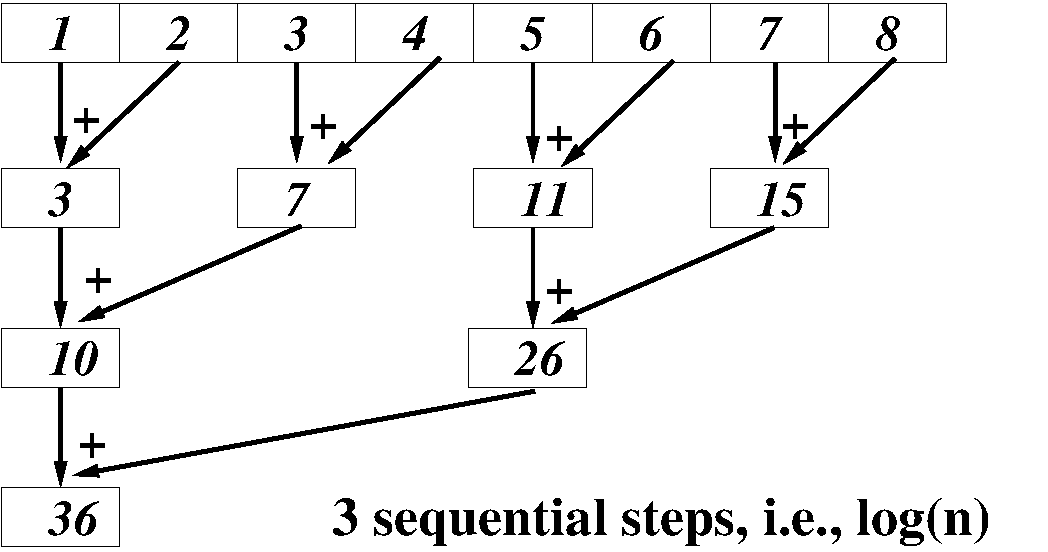
\includegraphics[height=25ex]{Figures/ReduceEg.pdf} 
\end{center} 

Build programs by combining \emp{map}, \emp{reduce} and other such operators. %Example: \smallskip

\end{frame}


\begin{frame}[fragile,t]
  \frametitle{1st List-Homomorphism Theorem [Meertens]}

\begin{columns}
\column{0.45\textwidth}
\begin{colorcode}[fontsize=\small]
h [ ]   = e
h [x]   = f(x)
h (x ++ y) = (h x) \mymath{\odot} (h y)
\end{colorcode}
\column{0.52\textwidth}
\begin{colorcode}[fontsize=\small]
h  \mymath{\equiv}  (reduce \mymath{\odot} e) \mymath{\circ} (map f)
\end{colorcode}
\end{columns}
\medskip

\emp{\bf Important Note: $\odot$ needs to be associative and $e$ needs to be the neutral element of $\odot$!}
\bigskip
\pause

\begin{columns}
\column{0.45\textwidth}
\begin{colorcode}[fontsize=\small]
-- one :: Int -> Int,one(x)=1
len :: [T] -> Int
len [ ]    = \emp{0}
len [x]    = \emp{one} x \blue{-- \mymath{\equiv} 1}
len (x ++ y) = (len x) \emp{+} (len y)
\end{colorcode}
\column{0.52\textwidth}
\begin{colorcode}[fontsize=\small]
    len \mymath{\equiv}\pause  (reduce (+) 0) \mymath{\circ} 
            (map one)
\end{colorcode}
\end{columns}


\bigskip
\begin{columns}
\column{0.45\textwidth}
\begin{colorcode}[fontsize=\small]
all\mymath{\myindx{p}} [ ]  = True
all\mymath{\myindx{p}} [x]  = p(x) 
all\mymath{\myindx{p}} (x++y) = (all\mymath{\myindx{p}} x) && (all\mymath{\myindx{p}} y)
\end{colorcode}
\column{0.52\textwidth}
\begin{colorcode}[fontsize=\small]
    all\mymath{\myindx{p}} \mymath{\equiv}\pause  (reduce (&&) True) \mymath{\circ} 
             (map p)
\end{colorcode}
\end{columns}


\end{frame}


\begin{frame}[fragile,t]
  \frametitle{List Homomorphism Invariants}

\begin{mytheo}[List-Homomorphism Promotions]\label{LHomInv}
Given unary functions $f$, $g$ and an associative binary operator $\odot$ then:\\
%$\mbox{ }$ \\
\emp{1.}$\ \ ({\tt map} \ f) \ . \ ({\tt map} \ g) \ \ \equiv \ \ {\tt map} \ (f \ . \ g)$\\
$\mbox{ }$ \\
\emp{2.}$\ \ ({\tt map} \ f) \ . \ ({\tt reduce} \ ({\tt ++}) \ []) \ \equiv \ ({\tt reduce} \ ({\tt ++}) \ []) \ . \ ({\tt map} \ ({\tt map} \ f) )$ \\
$\mbox{ }$ \\
\emp{3.}$\ \ ({\tt reduce} \ \odot \ e_{\odot}) \ . \ ({\tt reduce} \ (++) \ []) \ \equiv$\\
$ \ \ \ \ \ \ \ \ \ \ \ \ \ \ \ \ \ \ \ \ \ \ \ \ \ \ \ \ \ \ \ \ \ \ \
({\tt reduce} \ \odot \ e_{\odot}) \ . \ ({\tt map} \ ({\tt reduce} \ \odot \ e_{\odot}) )$
\end{mytheo}

%  

\begin{itemize}
    \item \emp{2. 3. $\Rightarrow$ code generation:} list is segmented, 
            segments are distributed on different processors, 
            computation proceeds locally on each processor, 
            and the local results are reduced. 
    \item \emph{2. 3. $\Leftarrow$ flattening optimization}: 
            uncovers more parallelism
    \item e.g., map f [1..4] = (map f) . (red ++) [[1,2],[3,4]] =$^{prom2}$ \alert{?}           
%(red ++) . (map (map f)) [[1,2], [3,4]] = \\red ++ [map f [1,2], map f [3,4]]
\end{itemize}

\end{frame}


\begin{frame}[fragile,t]
  \frametitle{Optimizing Map-Reduce Computation (\alert{Exercise})}

\begin{mytheo}[Optimized Map Reduce]\label{MapRed}
Assume {\tt distr$_p :: [\alpha] \rightarrow [[\alpha]]$}
distributes a list into $p$ sublists, each containing about 
the same number of elements. Denoting  
${\tt redomap }\ \odot \ f \ e_{\odot} \ \equiv \ ({\tt reduce} \ \odot \ e_{\odot}) \ . \ (map \ f)$, the equality holds:\\\bigskip

\emp{${\tt redomap} \ \odot \ f \ e_{\odot} \ \ \equiv$}\\
\emp{$\ \ \ \ \ \ \ \ \ \ \ \ \ \ \ \ \ \ \ ({\tt reduce} \ \odot \ e_{\odot}) \ . \ ({\tt map} \ ({\tt redomap} \ \odot \ f \ e_{\odot})) \ . \ {\tt distr}_p$}
\end{mytheo}

\begin{itemize}
    \item \alert{Prove it using the promotion Lemmas before!}
    \item \emph{Hint: $({\tt reduce} \ (++) \ []) \ . \ {\tt distr}_p \ \ \equiv \ \ id$, hence}
    \item \emph{${\tt redomap }\ \odot \ f \ e_{\odot} \ \equiv$\\ $\ \ \ \ ({\tt reduce} \ \odot \ e_{\odot}) \ . \ (map \ f) \ . \ ({\tt reduce} \ (++) \ []) \ . \ {\tt distr}_p$}
\end  {itemize}

\end{frame}

\subsection{Almost Homomorphisms Gorlatch'96}

\begin{frame}[fragile]
	\tableofcontents[currentsubsection]
\end{frame}

\begin{frame}[fragile,t]
  \frametitle{Maximum Segment Sum Problem (MSSP)}

\emp{``Systematic Extraction and Implementation of Divide-and-Conquer Parallelism'', Sergei Gorlatch, 1996.} 
\bigskip

\emph{Intuition}: a non-homomorphic function $g$ can be sometimes lifted 
to a homomorphic one $f$, by computing a baggage of \emp{\em extra info}. 

\bigskip

The initial fun obtained by projecting the homomorphic result:\\
$g\mbox{ }=\pi~\circ~f$

\bigskip

\emp{\bf Maximum-Segment Sum Problem ({\sc mssp})}: \\
Given a list of integers, find the contiguous segment of the list 
whose members have the largest sum among all such segments.\\
The result is only the maximal sum (not the segment's members).
For simplicity lets assume we are interested only in {\bf positive sums}.

\bigskip

E.g., {\tt mss} [1, -2, 3, 4, -1, 5, -6, 1] = 11 \\
(the corresponding segment is [3, 4, -1, 5]). 

\end{frame}


\begin{frame}[fragile,t]
  \frametitle{MSSP: Preliminary Reasoning}

\emp{\bf Maximum-Segment Sum Problem ({\sc mss})}: \\
Given a list of integers, find the contiguous segment of the list 
whose members have the largest sum among all such segments.\\
The result is only the maximal sum (not the segment's members).
For simplicity lets assume we are interested only in {\bf positive sums}.
\medskip

\red{A first straightforward/naive attempt:}
\begin{colorcode}
mss [ ]      = 0
mss [a]      = a \mymath{\uparrow} 0  \emp{//\mymath{\uparrow} denotes Max}
mss (x{\tt ++}\mbox{ }y) = mss(x) ??? mss(y)
\end{colorcode}

\bigskip
\bigskip

\begin{columns}
\column{0.58\textwidth}\pause
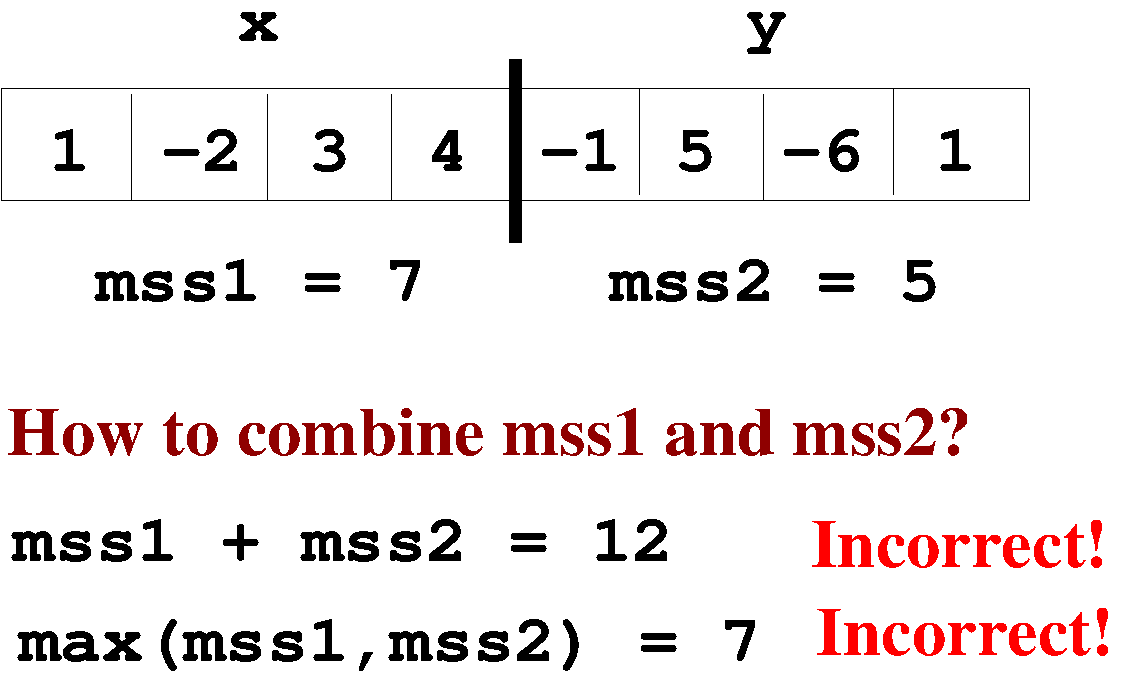
\includegraphics[height=20ex]{Figures/L1/mssp1}
\column{0.44\textwidth}
\red{Which case is problematic?}\pause\bigskip

\emph{Answer: when the segment of interest lies partly in {\tt x} and partly in {\tt y}!}
\end{columns}
\end{frame}

\begin{frame}[fragile,t]
  \frametitle{MSSP: A Better Reasoning}

\red{The problematic case is when the segment of interest lies
     partly in {\tt x} and partly in {\tt y}!}
\bigskip

We need to compute extra information:\pause
\begin{itemize}
    \item maximum concluding segment
    \item maximum initial segment
    \item total segment sum
\end{itemize}\smallskip\pause

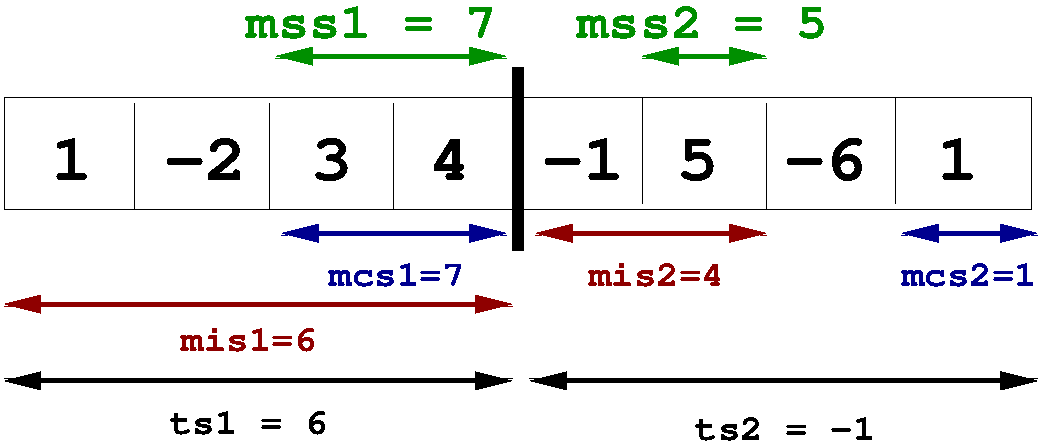
\includegraphics[height=22ex]{Figures/L1/mssp2}

\end{frame}

\begin{frame}[fragile,t]
  \frametitle{MSSP: Deriving the Implementation}

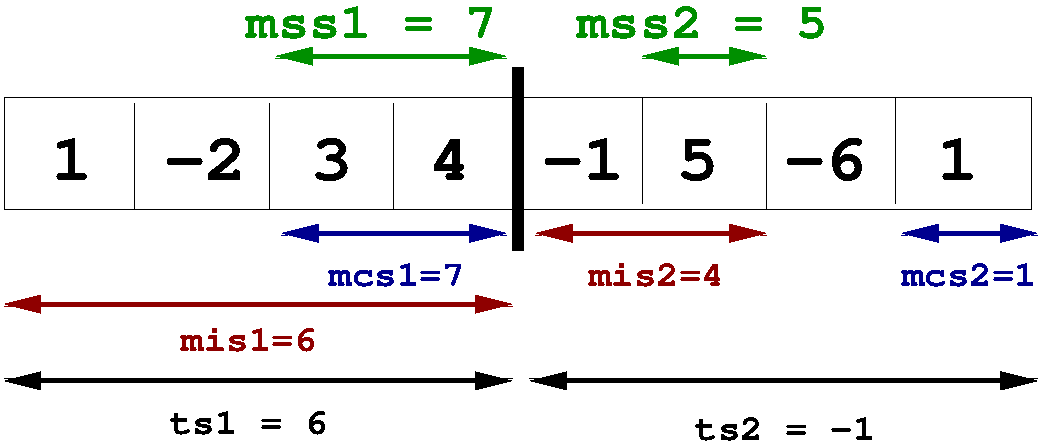
\includegraphics[height=22ex]{Figures/L1/mssp2}
\medskip
Lets compute the {\tt mis}, {\tt mcs}, {\tt mss}, and {\tt ts} for
the result of the two concatenating segments. $\uparrow$ denotes {\tt max}.

\bigskip
{\tt mis = \pause mis1 $\uparrow$ (ts1 + mis2)}
\medskip

{\tt mcs = \pause mcs2 $\uparrow$ (mcs1 + ts2)}
\medskip

{\tt mss = \pause mss1 $\uparrow$ mss2 $\uparrow$ (mcs1 + mis2)}
\medskip

{\tt ts~~= ts1 + ts2}
\end{frame}


\begin{frame}[fragile,t]
  \frametitle{Maximum-Segment Sum = Near Homomorphism}

\begin{block}{Correct Solution (Haskellish)}
\begin{colorcode}
-- \mymath{x\mbox{ }\uparrow\mbox{ }y = if(x >= y) then x else y}
(mssx, misx, mcsx, tsx) \mymath{\odot} (mssy, misy, mcsy, tsy) = (
        (mssx\mymath{\mbox{ }\uparrow\mbox{ }}mssy\mymath{\mbox{ }\uparrow\mbox{ }}(mcsx+misy),
         misx\mymath{\mbox{ }\uparrow\mbox{ }}(tsx+misy),
        (mcsx+tsy)\mymath{\mbox{ }\uparrow\mbox{ }}mcsy,
         tsx + tsy
    )

f x = (x\mymath{\mbox{ }\uparrow\mbox{ }}0, x\mymath{\mbox{ }\uparrow\mbox{ }}0, x\mymath{\mbox{ }\uparrow\mbox{ }}0, x)

\emph{emss = (reduce \mymath{\odot} (0,0,0,0)) . (map f)}

\emp{mss  = \mymath{\pi\myindx{1}} . emss}
       where \mymath{\pi\myindx{1}} (a, _, _, _) = a 
\end{colorcode}
\end{block} 

\smallskip

The baggage: $3$ extra integers ({\tt misx, mcsx, tsx}) 
and a constant number of integer operations per communication stage. 

%Optimal time and work complexity with $N/log(N)$ processors.

\end{frame}


\begin{frame}[fragile,t]
  \frametitle{Longest Satisfying Segment Problems}

\begin{itemize}
    \item Class of problems which requires to find the longest segment of a list
            for which some property holds, such as:
    \item longest sequence of zeros, or longest sequence made from the same number, or longest sorted sequence.  
    \item Not all predicates can be written as a list homomorphism, e.g., longest sequence whose sum is 0.
\end{itemize}

\bigskip

\begin{block}{Restrict The Shape of the Predicate to:}
\begin{colorcode}
p []           = True
p [x]          = ...
p [x, y]       = ...
p [x : y : zs] = (p [x,y]) \mymath{\wedge} p (y : zs)
\end{colorcode}
\end{block} 

\end{frame}


\begin{frame}[fragile,t]
  \frametitle{Longest Satisfying Segment Problems}

\begin{block}{Restrict the Shape of the Predicate:}
\begin{colorcode}
zeros [x]   = x == 0           same [x]   = True     sorted [x]   = True
zeros [x,y] =  (zeros [x])     same [x,y] = x == y   sorted [x,y] = x <= y
             \mymath{\wedge} (zeros [y])
\end{colorcode}
\end{block} 

\bigskip
Extra Baggage:
\begin{itemize}
    \item As before, the \emp{length} of the longest initial/concluding  satisfying segments ({\tt lis}/{\tt lcs}),
            and the total list length ({\tt tl}).
    \item When considering the concatenation of the {\tt (lcs, lis)} pair, it is not guaranteed that the
            result satisfies the predicate, e.g., 
            {\tt (sorted x) $\wedge$ (sorted y) $\not\Rightarrow$ sorted x++y}. \pause  
    \item We also need the {\em last} element of {\tt lcs} and the {\em first} elem of {\tt lis},
    \item in order to compute whether {\tt (lcs x)} is {\em connected} to {\tt (lis y)}, \\ i.e., {\tt p [lastx,firsty] == True}
%    \item Boolean indicating whether the whole list satisfies {\tt p} ({\tt ok}).
\end{itemize}
\end{frame}

\begin{frame}[fragile,t]
  \frametitle{Longest Satisfying Segment Problem: Exercise}

\begin{block}{Exercise: fill in the blanks, test in Haskell for zeros/same/sorted}
\begin{colorcode}
(lssx, lisx, lcsx, tlx, firstx, lastx) \mymath{\odot}
(lssy, lisy, lcsy, tly, firsty, lasty) 

  = (newlss, newlis, newlcs, tlx+tly, first, last)
     where
        connect = ...
        newlss  = ...
        newlis  = ... 
        newlcs  = ... 
        first   = if tlx == 0 then firsty else firstx
        last    = if tly == 0 then lastx  else lasty

f x = (xmatch, xmatch, xmatch, 1, x, x)
    where xmatch = if (p [x]) then 1 else 0

\emph{elss = (reduce (\mymath{\odot}) (0,0,0,0,0,0)) . (map f)}

\emp{lss  = \mymath{\pi\myindx{1}} . elss}
       where \mymath{\pi\myindx{1}} (a, _, _, _, _, _) = a         
\end{colorcode}
\end{block} 

%lssx \mymath{\uparrow} lssy \mymath{\uparrow} (if connect then ... else 0)
%+ (if okx \mymath{\wedge} connect then ... else 0)
%+ (if oky \mymath{\wedge} connect then ... else 0)
%okx \mymath{\wedge} oky \mymath{\wedge} connect

\end{frame}



%\begin{frame}[fragile,t]
%  \frametitle{Longest Satisfying Segment Problem -- Solution}
%
%\begin{block}{Longest Satisfying Segment Solution}
%\begin{colorcode}
%(lssx, lisx, lcsx, tlx, firstx, lastx, okx) \mymath{\odot}
%(lssy, lisy, lcsy, tly, firsty, lasty, oky) 
%
%  = (newlss, newlis, newlcs, tlx+tly, firstx, lasty, newok)
%     where
%        connect = p [lastx, firsty]
%        newlss  = lssx \mymath{\uparrow} lssy \mymath{\uparrow} (if connect then lcsx+lisy else 0)
%        newlis  = lisx + (if okx \mymath{\wedge} connect then lisy else 0)
%        newlcs  = lcsy + (if oky \mymath{\wedge} connect then lcsx else 0)
%        newok   = okx \mymath{\wedge} oky \mymath{\wedge} connect
%
%f x = (xmatch, xmatch, xmatch, 1, x, x, p [x])
%    where xmatch = if (p [x]) then 1 else 0
%
%-- In Haskell write \emp{red \mymath{(\odot)\mbox{ }e\myindx{\odot}}}, where \mymath{e\myindx{\odot} = (0,0,0,0,0,0,True)}
%\emph{elss = (red \mymath{\odot}) . (map f)}
%
%\emp{lss  = \mymath{\pi\myindx{1}} . elss}
%       where \mymath{\pi\myindx{1}} (a, _, _, _, _, _, _) = a         
%\end{colorcode}
%\end{block} 
%
%\end{frame}

\begin{frame}[fragile,t]
  \frametitle{Conclusion}

What have we talked about today?\bigskip
\begin{itemize}
    \item Hardware Parallelism:\pause\\ the only way of scalably increasing the compute power.\bigskip
    \item Big Challenge:\pause having parallel commodity software.\bigskip
    \item List-Homomorphism:\\ a way of reasoning about parallelism and\\ of building inherently parallel programs.  
\end{itemize}
\end{frame}


\end{document}
